\section{Test mit zusätzlichem Wissen} % 106 - 59
\label{sec:test_knowledge}

In Abschnitt \ref{sec:ana:rundenfunktion} (Abbildung \ref{eq:calcD}) wurde zusätzliches Wissen über die Rundenfunktion ermittelt/beschrieben.
Für einen SAT-Solver mag dieses Wissen redundant sein und überflüssig erscheinen, weil ein SAT-Solver nicht zwischen Vorwärts- und Rückwärts-Rechnen
unterscheidet. Jedoch werden durch dieses Wissen bestehende Module noch einmal anders verknüpft, was einem SAT-Solver die Möglichkeit bieten könnte,
einen alternativen Pfad zu nutzen und weitere Zusammenhänge zwischen Modulen zu erkennen. Nach dem selben Prinzip wäre es auch möglich, die Addition
von mehreren Summanden in unterschiedlicher Reihenfolge zusätzlich einzufügen. Der Fokus liegt jedoch darauf, nur festzustellen, ob sich das
zusätzliche Wissen überhaupt auswirkt, weshalb auf die zusätzlichen Addierer verzichtet wird.

Ein Unterschied zu den vorhergehenden Tests ist, dass bei diesem Test nicht nur zusätzliche Klauseln notwendig sind, sondern auch weitere Literale
benötigt werden. Außerdem wird ein zusätzliches Modul für die Subtraktion genutzt, welches bisher nicht näher beschrieben wurde, weil es nach dem selben
Prinzip wie ein Addierer aufgebaut ist.

Die Ergebnisse sind in Abbildung \ref{fig:data_know} dargestellt. Während sich bei den vorhergehenden Tests die Laufzeit generell verkürzt oder
verlängert hat, verhalten sich die beiden Varianten in diesem Tests entgegengesetzt. Während sich die Laufzeit bei der Variante ohne XOR-Klauseln
leicht verlängert hat, hat sie sich bei der Variante mit XOR-Klauseln um 40\% verkürzt. Bei beiden Varianten ist jedoch ersichtlich, dass sich die
Anzahl der unterschiedlichen Lösungen speziell im Bereich mit wenig vorgegeben Bits erhöht hat. Das deutet darauf hin, dass CryptoMiniSat wieder
mehr rät. Bei der Variante mit XOR-Klauseln hat das jedoch gut geklappt. Fraglich ist aber, ob das dem Zufall geschuldet ist.
\begin{figure}[!h]
  \centering
  \begin{minipage}[c]{0.45\textwidth}
  \begin{flushleft}Gesamtdauer ohne XOR: 205:09:48\end{flushleft}
  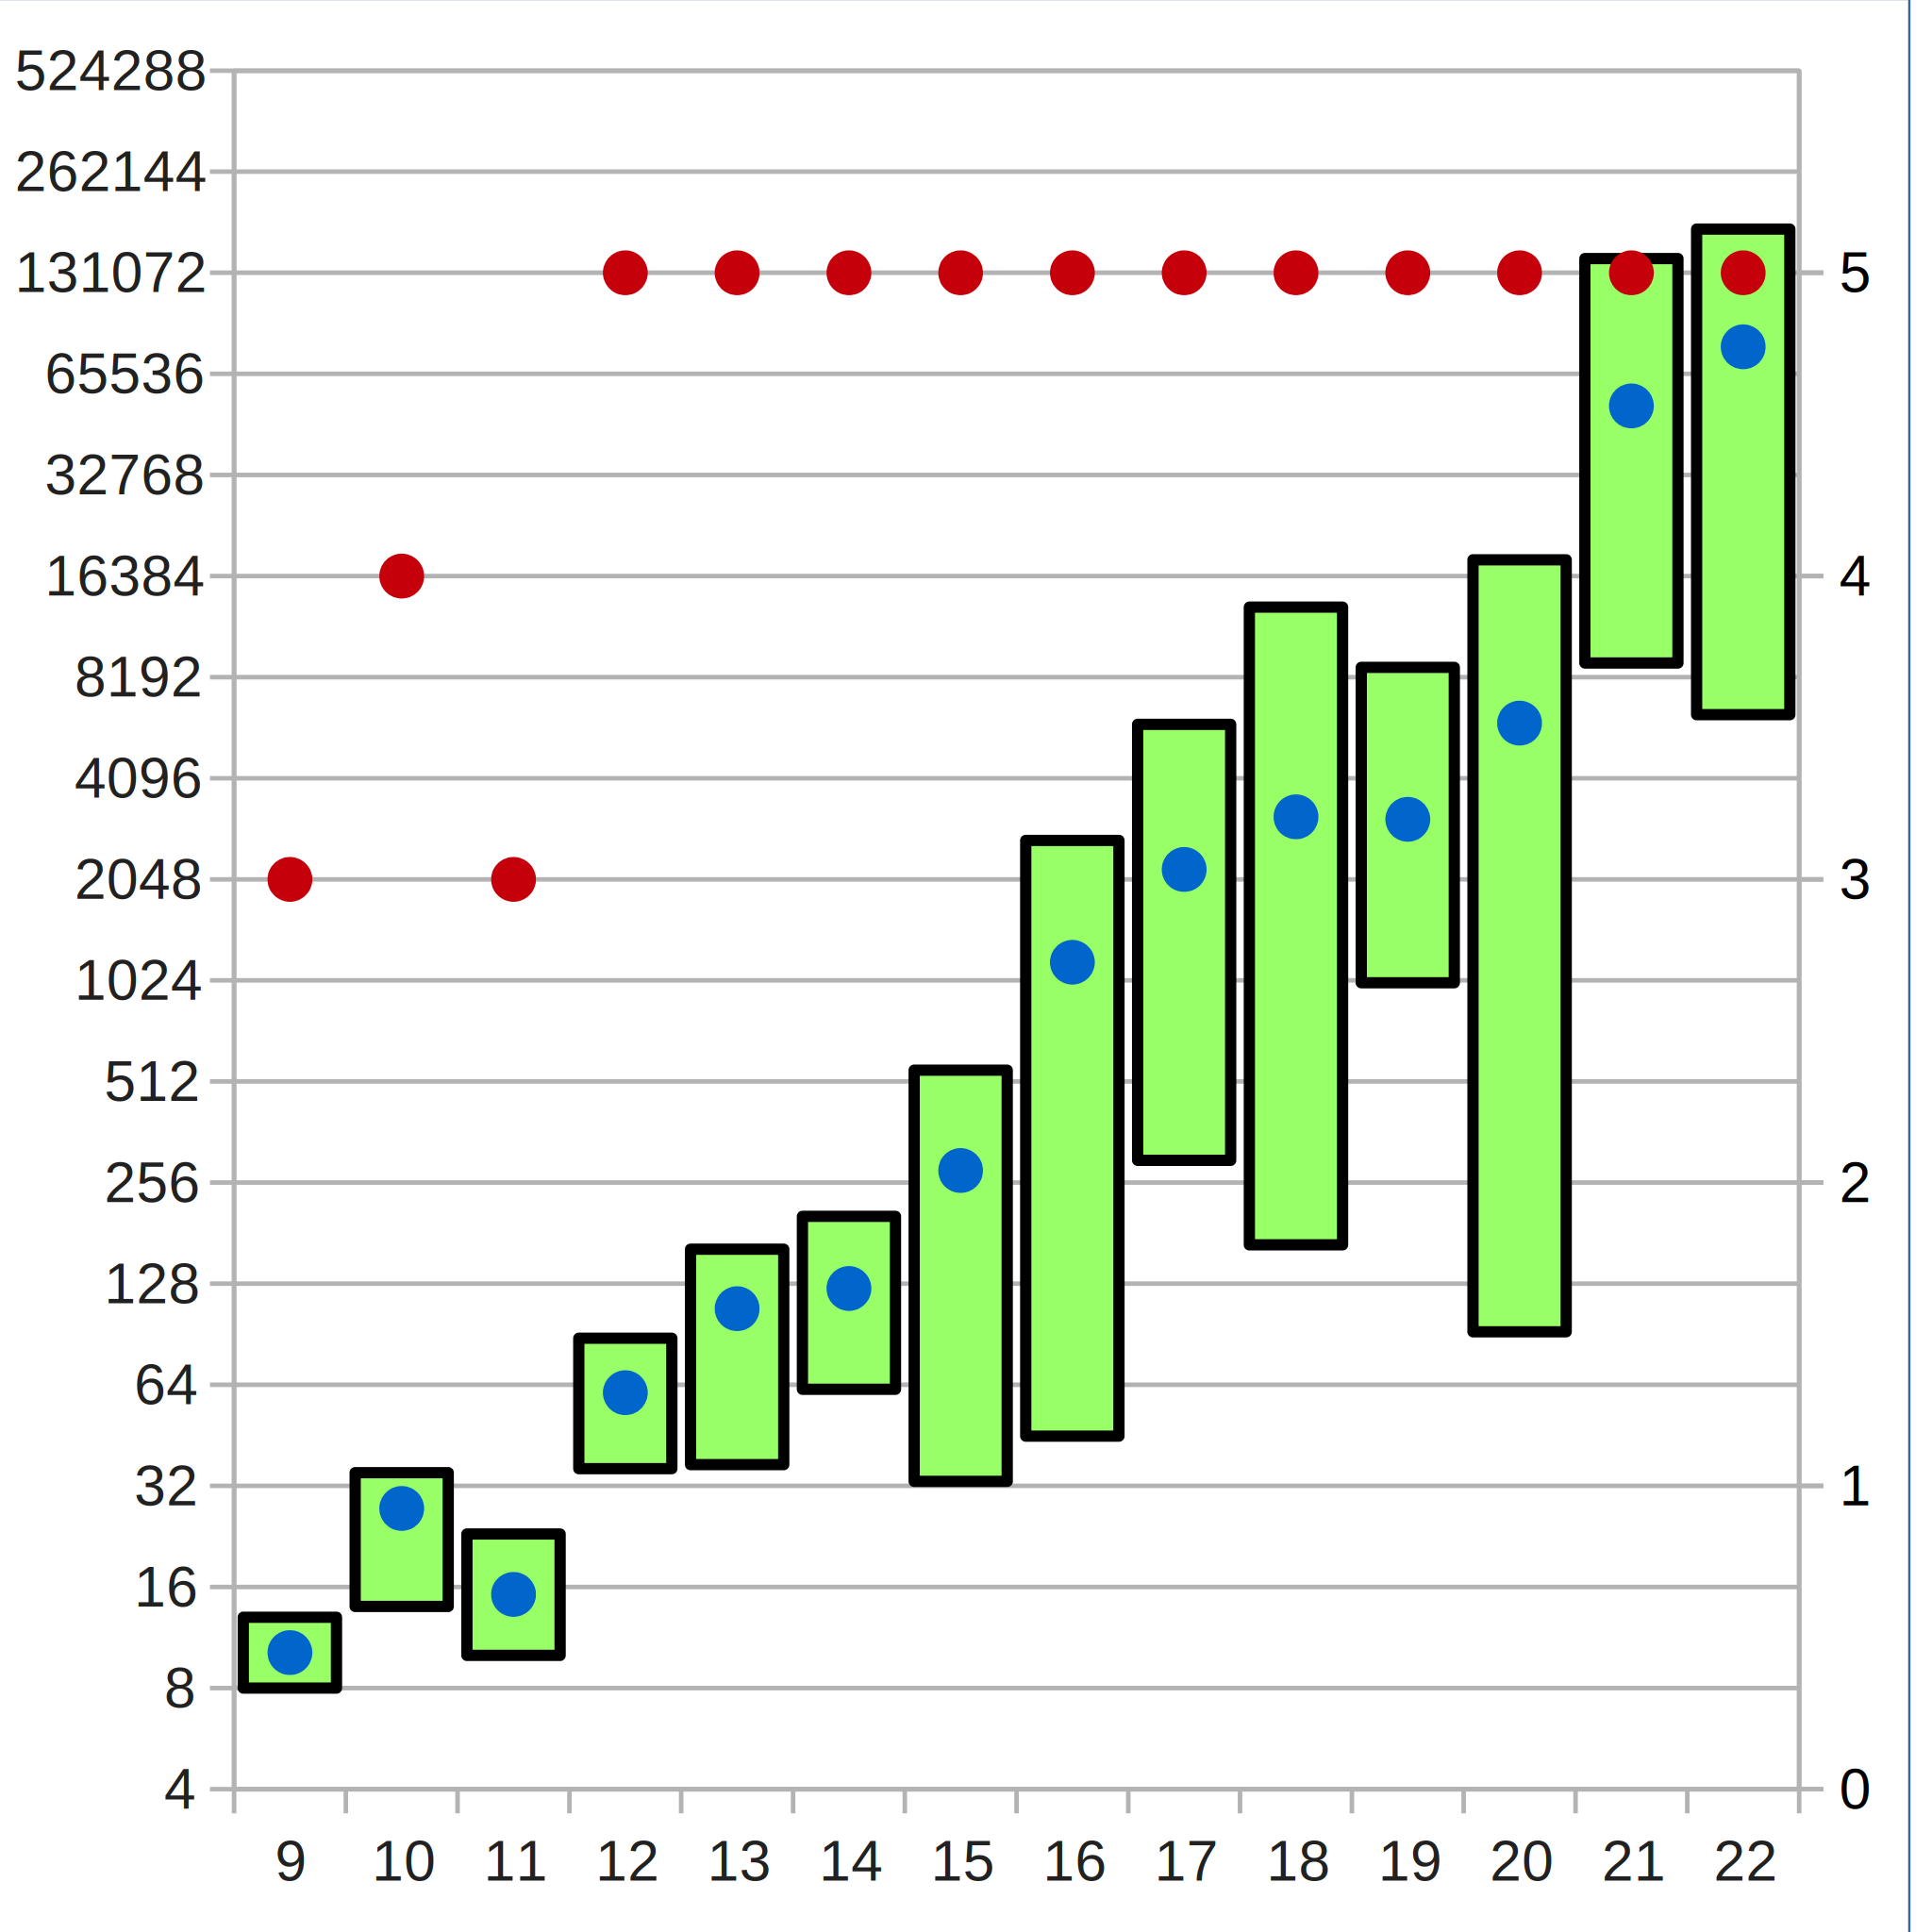
\includegraphics[scale=0.55]{images/data_know_knf}
  \end{minipage}
  \begin{minipage}[c]{0.09\textwidth}
  ~~
  \end{minipage}
  \begin{minipage}[c]{0.45\textwidth}
  \begin{flushleft}Gesamtdauer mit XOR: 100:41:09\end{flushleft}
  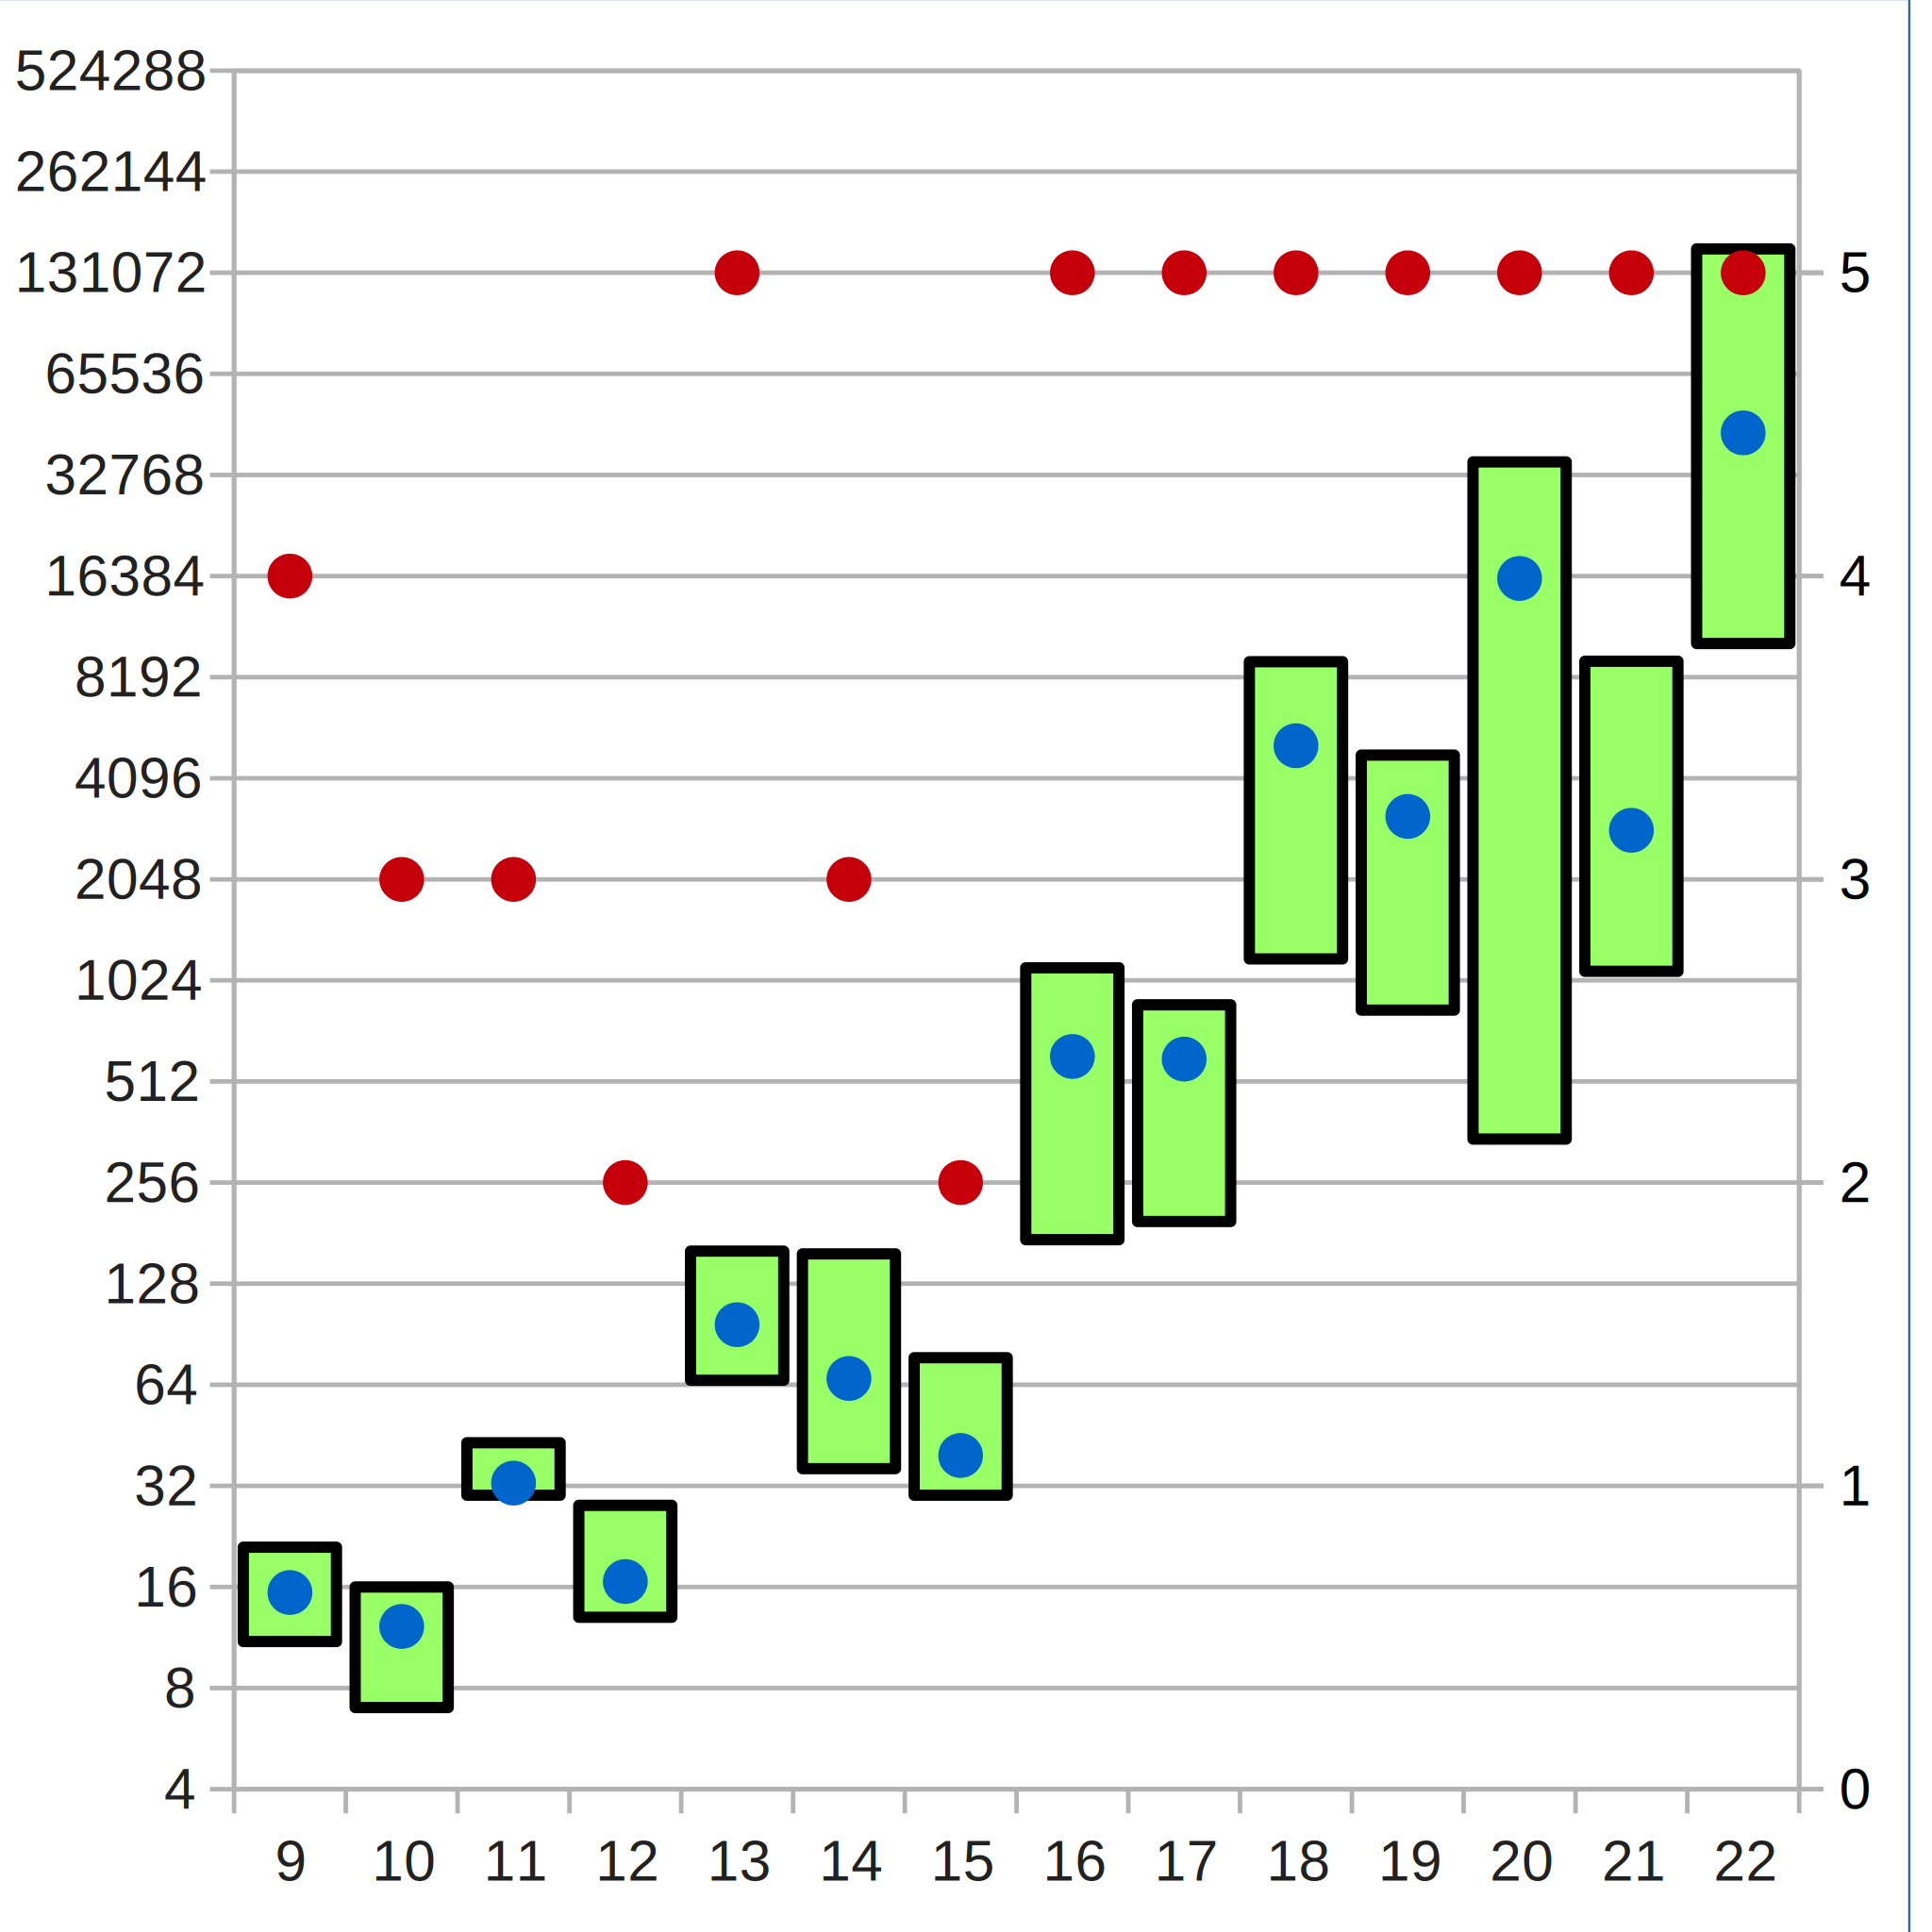
\includegraphics[scale=0.55]{images/data_know_xor}
  \end{minipage}
  \caption{Ergebnisse mit zusätzlichem Wissen}
  \label{fig:data_know}
\end{figure}